
\chapter{曲线运动}
\section{教学要求}
这一章讲授平抛、斜抛和匀速圆周运动,是牛顿运动定律
在“新”的领域的具体运用,速度和加速度的方向性,在曲线
运动显得非常重要,通过本章的学习,学生对这两个概念的矢
量性将得到进一步的领会。

这一章的教学要求是:
\begin{enumerate}
\item 了解曲线运动的特点和物体做曲线运动的条件,掌握
运动的合成与分解的方法。
\item 理解平抛运动和斜抛运动的规律,会用运动的合成与
分解的方法分析这两种运动。
\item 理解匀速圆周运动的角速度、线速度和周期的概念,
掌握它们之间的关系$v=r\omega=\dfrac{2\pi r}{T}$
\item 掌握向心加速度的概念,会用向心加速度的公式.掌
握向心力的概念,会分析做匀速圆周运动的物体的受力情况,
找出向心力的来源。
\item 了解离心现象及其应用。
\end{enumerate}

下面对这一章的教学内容作些具体说明。

关于曲线运动的一般特点,主要说明曲线运动中速度的
方向是时刻变化的,因此,曲线运动都是变速运动,对于曲线
运动的速度方向,教材是通过分析现象得出的,没有从数学上
进行论证,这是考虑到这种讲法比较简单易懂,便于学生接
受。关于物体做曲线运动的条件,要求学生知道,但不要求进
一步分析合外力对速度的大小和方向的影响。程度好一些的
学生,可以在学完第七节后,通过阅读材料“力的分解与曲线
运动”,来加深对这个问题的理解。

运动的合成和分解是作为研究平抛和斜抛的方法来讲解
的。因为是准备性知识,所以讲得比较简要。要求学生掌握
运动的合成和分解的方法,但不要求进行论证。教材是对同
一参照物来讲解运动的合成和分解的,不涉及相对速度、牵连
速度等概念。课本里提到的运动都是相对于地面来说的,不
会误解,所以没有把参照物写出来。

关于平抛和斜抛运动,主要是要使学生认识抛体运动可
以看作是竖直方向和水平方向两个直线运动的合运动。对于
计算飞行时间、射程和射高的公式,主要要求学生知道它们是
怎样推导出来的,掌握推导方法,而不要死记硬背。平抛和斜
抛运动的轨迹曲线,教材是用描点法画出的,不要求由已给
出的时间参数方程推导出用$x$和$y$表示的抛物线方程。

角速度和周期这两个描述匀速圆周运动快慢的物理量,
学生初次接触,应使学生理解它们的物理意义。同时还应要
求学生搞清楚线速度、角速度、周期这三个量是从不同角度
来描述匀速圆周运动快慢的,并掌握它们之间的关系。匀速
圆周运动的线速度的大小虽然不变,但方向却时刻在改变,因
而匀速圆周运动是变速运动,认识这一点是后面讲解向心加
速度的前提。

关于向心加速度,教材是用矢量方法讲的。这种讲法能
突出向心加速度的方向,有利于学生正确理解向心加速度,对
向心加速度的推导学生只要能听懂就行,并不要求学生自己
会推导。由于全书都不写矢量式,这里也没有用矢量式。为
了避免用矢量差,采用学生学过的矢量合成的三角形法,用
$v_B$等于$v_A$与$\Delta v$之和的提法代替了$\Delta \vec{v}=\vec{v}_B-\vec{v}_A$, 不同的教师
可能爱好的推导方法不一样,在教学中可以不必拘泥于课本
中的方法,根据自己的爱好选用其他的推导方法。

导出向心加速度的公式后,应使学生知道匀速圆周运动
是变加速运动,对于不同形式的向心加速度公式:$a_n=\dfrac{v^2}{r}$
和
$a_n=\omega^2 r$, 应使学生了解它们的物理意义,知道在什么条件下
$a_n$与$r$成反比,在什么条件下$a_n$与$r$成正比;并能利用$v$、$\omega$、
$r$之间关系,从一种形式推导出另一种形式,以备后面学习中
应用。

讲解向心力时,应突出牛顿运动定律的应用。向心力的
大小可由牛顿第二定律算出,向心力的方向跟加速度的方向
时刻都是一致的,总是指向圆心,在分析向心力问题时,也应
注意强调从牛顿运动定律出发进行研究。

分析向心力的来源是一个难点,又是理解和掌握向心力
的关键。为此教材写了“匀速圆周运动的实例分析”一节,就
一些实际的例子分析了向心力的来源,以及向心力的大小跟
物体做匀速圆周运动情况的关系。并且,使学生进一步明确:
使物体做匀速圆周运动的向心力就是物体受到的合外力。

“离心现象”一节主要是使学生了解物体做离心运动的原
因和离心机械的原理。

\section{教学建议}
本章可分为三个单元进行教学,第一单元是第一节《曲线
运动》,第二单元从第二节《运动的合成和分解》到第四节《斜
抛物体的运动》,第三单元从第五节《匀速圆周运动》到第九节
《离心现象》。

\subsection{第一单元}
这一单元是整章的讨论前提与研究曲线运动的基础,主
要使学生认识曲线运动中的速度方向是时刻改变的,获得曲
线运动是变速运动的印象以及正确理解物体做曲线运动的
条件。

\subsubsection{曲线运动的速度方向}

关于曲线运动的速度方向,课
本是通过图4.2所示的现象得出结论的.在分析这个现象时
要使学生认识,即使刀具不跟砂轮接触,砂粒没有落下,也没
有火星飞出,砂轮边缘上各点做圆周运动的速度方向,仍然
是在儡周各点的切线方向上。认清了这一点之后,再进一步引
导学生明确曲线运动是一种变速运动,为进一步学习物体做
曲线运动的条件做好准备。

\subsubsection{物体做曲线运动的条件}

讲这部分内容时先明确一下,
曲线运动既然是变速运动,运动
物体所受的力一定是不平衡的。
然后做一个演示实验(图4.1):
一个乒乓球在水平桌面上沿着一条直线滚动到桌子边缘的$B$
点。当乒乓球离开桌边后,由于在竖直方向上受到重力的作
用,就改变了原来的直线运动状态,沿着曲线$BCD$运动了,再
分析乒乓球的受力情况,使学生认识物体做曲线运动的条件
是:物体具有初速度,并且受到跟初速度方向成一角度(不包
括$0^{\circ}$和$180^{\circ}$这两种特殊情况)的合外力的作用。

\begin{figure}[htp]
    \centering
\includegraphics[scale=.5]{fig/4-1.png}
    \caption{}
\end{figure}

\subsection{第二单元}
这一单元学习运动的合成和分解以及平抛和斜抛物体的
运动。把复杂的运动看成由两个或几个比较简单的分运动所
组成,是这一单元中要学习的一种重要的分析研究问题的
方法。

\subsubsection{运动的合成和分解}

学生对轮船渡河的现象可能缺
乏感性认识,可以先做一个简单的演示(详见本章实验指导)
加以说明,然后再分析课本所讲的例子。

在讲解运动的合成和分解时,可以向学生说明分运动的
性质决定了合运动的性质与合运动的轨迹。如果物体的两个
分运动都是匀速直线运动,则合运动必定也是匀速直线运动,
合运动的位移和分运动位移间的关系符合平行四边形法则。
而且合运动的位移等于合运动的路程。如果物体的两个分运
动,互成一定角度,其中一个是匀速直线运动,另一个是变速
运动,则合运动是变速运动,而且运动轨迹必定是曲线。合运
动的位移仍能用平行四边形法则进行计算,但是合运动位移
并不等于合运动轨迹的长度——路程。

\subsubsection{平抛物体的运动}

讲解平抛运动时,在演示实验(详见本章实验指导)和对课本图4.10的闪光照片进行分析的基
础上,应使学生认识以下几点。

平抛运动是水平方向的匀速直线运动和竖直方向的
自由落体运动的合运动.根据课本图4.9的实验,两个小球
同时落地的事实,得出平抛运动在竖直方向上的分运动是自
由落体运动的结论,而对课本图4.10的闪光照片进行分析的
结果可以证明做平抛运动的小球在水平方向上的分运动是匀
速直线运动。

为了加深学生对平抛运动的这两个分运动的认识,也可
以再从理论上进行分析:如果小球在做平抛运动之前是在一
个光滑的水平面上运动,则根据牛顿第一定律可知,小球将保
持它的匀速直线运动状态不变,而当小球离开光滑水平面后,
在水平方向上没有受到任何力(忽略空气阻力)的作用,于是
它将继续保持做匀速直线运动。而在竖直方向上,由于小球
不再受到水平面支持力的支托,它将在重力作用下产生加速
度,做初速度等于零、加速度等于$g$的匀变速直线运动。

平抛运动的飞行时间和水平距离。在讨论平抛运动
的公式时,应使学生注意,平抛物体的飞行时间$t$受到下降距
离$y$的限制,$t=\sqrt{\dfrac{2y}{g}}$
譬如让两个身高不同的同学推铅球,假
定他们推出的铅球初速度都在水平方向上,而且大小相等,显
然他们能使铅球做平抛运动的时间是不相等的,高个同学推
出的铅球做平抛运动的时间长些,推出的铅球飞行的水平距
离也将大些。所以说,平抛运动的时间$t$决定于自由下落的
距离$y$, 而水平距离$x$则跟平抛初速$v_0$和飞行的时间$t$都有
关系。

平抛物体的落地速度.
在讨论平抛物体的落地速度
时,要让学生了解,落地速度
是水平方向分速度和竖直方向分速度的合速度,这一速度的
方向应在其运动轨迹这一点的
切线方向上,如图4.2所示.因
此是不可能垂直于地面的。如果落地速度$v$和水平方向夹角为$\theta$, 则\[\tan\theta= \frac{v_y}{v_x}=\frac{\sqrt{2gy}}{v_0} \]
在求矢量的运算中,有的同学往往只注意求出矢量的大小,忘记
了求出矢量的方向。这是初学者易犯的通病,可以结合平抛
物体落地速度的计算,提醒他们注意这个问题。

\begin{figure}[htp]
    \centering
\includegraphics[scale=.5]{fig/4-2.png}
    \caption{}
\end{figure}

还应该使同学们了解,对于落地点的即时速度的讨论同
样适用于平抛运动轨迹上的任一点。

\subsubsection{斜抛物体的运动}

在做好课本图4.14演示实验的
基础上,使学生认识以下几点:
\begin{enumerate}
\item 可以把斜抛运动看成是水平方向的匀速直线运动和
竖直方向的上抛运动的合运动。
\item 斜抛运动具有一定的对称性,这包括物体到达最高
点的时间与从最高点落回到地面的时间相等,初速度的大小
与落地时的末速度的大小相等,抛射角与到达落地点时末
速度与水平面间的夹角相等。
\item 做斜抛运动的物体在到达最高点以后的运动是平抛
运动,因此平抛运动可以看成是斜抛运动的一部分。
\item 不论是平抛运动还是斜抛运动,物体都具有跟重力
方向成一角度的初速,并且是只在重力作用下的运动。因此
它们的共同点表现为运动的加速度都等于重力加速度$g$, 运
动中的速度变化,都发生在竖直方向上。
\end{enumerate}

\subsection{第三单元}
这一单元主要讲匀速圆周运动,是本章的教学重点。
\subsubsection{描述匀速圆周运动快慢的几个物理量}
要使学生认
识用线速度来比较质点做匀速圆周运动的快慢时,质点运动
的圆周半径必须相同的。而用周期和角速度来描述匀速圆
周运动的快慢程度时,则不必考虑圆周的半径。这两种不同
的描述方法,各有它们的长处,在以后的学习中将根据讨论问
题的方便选用不同的描述方法。

课本练习五第4题提到的“每分钟的转数$n$”同
样可以描述匀速圆周运动的快慢程度。为了使学生更具体地
理解这一点,可以比较指针式手表上三个指针的运动,秒针的
转数最大,$n_1=1$转/分,分针的转数$n_2=\frac{1}{60}
$转/分,而时针的转
数最小,$n_3=\frac{1}{720}$
转/分。因此秒针上的质点(除转轴外)做匀速
圆周运动转动最快,而不论这些质点离开转轴距离的大小
如何。

\subsubsection{匀速圆周运动是变速运动}

在匀速圆周运动中,周期
和角速度这两个量是不随时间而改变的。线速度则是随时间
变化的。这一点有的同学不易接受,关键在于忽略了速度是
个矢量。线速度的大小虽然不变,但它的方向却是时刻改变
的。匀速圆周运动中的“匀速”,是指线速度的大小不变而
言的。

\subsubsection{匀速圆周运动中的向心加速度}

要使学生正确认识向
心加速度公式的两种表达式$a_n=v^2/r$
和$a_n=\omega^2 r$的物理意义,
在利用这两个公式来比较两个做匀速圆周运动的质点的向心
加速度的大小时,能搞清当线速度$v$相等时,向心加速度$a_n$, 跟
运动半径$r$成反比;当角速度$\omega$相等时,向心加速度$a_n$跟运
动半径$r$成正比。这一点可以结合自行车的传动装置来说明:
跟踏脚板连在一起的链轮边缘质点的线速度$v$和飞轮边缘质
点的线速度$v$是相等的,由于链轮的半径大于飞轮的半径,因
此链轮边缘质点的向心加速度小于飞轮边缘质点的向心加速
度。而飞轮和自行车后轮是同轴装置的,它们的角速度$\omega$相
等,所以后轮边缘质点的向心加速度大于飞轮边缘质点的向
心加速度。

\subsubsection{向心力}

向心力的教学,要使学生认识如下几个问题:
\begin{enumerate}
\item 在匀速圆周运动中必定有产生向心加速度的向心
力。要强调指出,向心力是根据力的效果来命名的,而不是根
据力的性质来命名的,因此,它不是重力,弹力、摩擦力等以外
的特殊的力,而是做匀速圆周运动的质点受到的合外力,沿着
半径指向圆心,它的方向时刻改变,因此产生向心加速度的
力——向心力也是始终沿着半径指向圆心的,它是一个变力。
\item 质点做匀速圆周运动的条件是:质点具有初速度$v$,
并且始终受到跟线速度方向垂直,大小等于
$mv^2/r$的合外力(即向心力)的作用。
\end{enumerate}

\subsubsection{做匀速圆周运动物体的受力分析}

确定物体所需的
向心力的来源,是研究匀速圆周运动的关键.课本图4.20、
4.21、4.22、4.24和4.27所分析的五个例子都是物体在水平
面上做匀速圆周运动的情况,因此它们受力情况的共同点是:
不论物体受几个力的作用,合力一定是在水平方向,沿着半径
指向圆心的,这一合力就是使物体做圆周运动所需的向心力。
在进行具体例子的分析时,要引导学生注意如下两点:

\begin{enumerate}
\item 要判断圆心的位置和
质点做圆周运动的半径,例如
在北京的物体随地球自转做匀
速圆周运动的圆心位置并不是地球的中心,而是从北京的纬
度处作地轴的垂线的垂足$O$(图
4.3). 而这一垂线的长度就是
在北京的物体做圆周运动的半
径$r=R\cos40^{\circ}$. 又如在圆锥摆的运动中(图
4.24), 小球做匀速圆周运动的圆心位置在圆锥底面的中心,
而不是悬绳上端的固定点,小球的运动半径是圆锥底面的半
径,而不是悬绳的长度。
\item 对物体进行受力情况分析时,要求作出受力图,然后
根据牛顿第二定律来确定加速度和力的关系。
\end{enumerate}

\begin{figure}[htp]
    \centering
    \includegraphics[scale=.5]{fig/4-3.png}
    \caption{}
\end{figure}


\subsubsection{离心现象}

在讲解离心运动时,要注意明确两点:
\begin{enumerate}
    \item 离心运动不是由于受到“离心力”的作用,离心运动是惯性的表现。
    \item 做匀速圆周运动的物体在合外力突然消失后,不是
    沿着半径方向“离心”而去的,而是沿着失去向心力的这一位
    置时的切线方向飞出。
\end{enumerate}

因此对于课本图4.28应有如下的理解:
\begin{enumerate}
    \item 这是一个示意图,为了便于比较,把三种情况画在同
一个图中。
\item 图中离开圆心$O$距离最近的一个小球,是能够沿着
原来的圆弧做匀速圆周运动的,所需的向心力能够得到满足,
这是正常的情况。
\end{enumerate}

离开圆心$O$距离稍远的一个小球,是表示由于向心力不
足,这一比较小的向心力将不能使小球沿着原来的半径继续
做圆周运动,在认为线速度$v$不变(由于惯性)的条件下,向心
力$F=mv^2/r$
减小后,从这一即时的情况来看,小球只能在曲率
半径$r$较大的一小段圆弧上运动。这样,对原来的圆心位置
来说,距离就远了。

离开圆心$O$最远的一个小球,是表示向心力突然消失,消
失的位置是在圆心$O$的正上方,因此小球将沿着切线方向
飞出。

后面的两种情况都是小球的离心运动。


\section{实验指导}
\subsection{演示实验}
\subsubsection{物体做曲线运动的条件}

如图4.4所示,利用投影仪观察,使一小铁球从斜槽上滚
下,小球将沿直线$OO'$运动,然后在垂直于$OO'$的方向上放
一块条形磁铁,使小球再次从斜槽上滚下后,它将偏离原来的
运动方向做曲线运动(演示时磁铁不要离$OO'$线太近,以免
小铁球被磁铁吸住)。


\begin{figure}[htp]
    \centering
    \includegraphics[scale=.5]{fig/4-4.png}
    \caption{}
\end{figure}

\subsubsection{运动的合成}
把一个注满水的乒乓球用细线系住,细线的另一端用图
钉固定在小黑板左侧的$B$点。放松细线,乒乓球静止在$A$点,
如图4.5甲所示,在小黑板上经过$B$点斜向上(方向任意)画
一直线$BB'$(注意使$BB'$的长度约等于$AB$间的距离)如图4.5
乙所示。
\begin{figure}[htp]
    \centering
    \includegraphics[scale=.5]{fig/4-5.png}
    \caption{}
\end{figure}

如果将食指勾在悬线的左侧,使手指沿着直线$BB'$移动,
便可观察到乒乓球同时参与从$A\to B$以及从$B\to B'$两个不同
方向的运动,而其实际运动轨迹的是沿着$A$点和$B'$点的连线
方向,如图4.5丙所示,从而说明两个匀速直线运动的合运
动仍是一个匀速直线运动,合运动位移和分运动位移的关系
符合平行四边形法则。

\subsubsection{自由落体和平抛物体同时落地}
课本图4.9的演示,为了使效果更好,可以使$B$球略
小于$A$球,或者设法将$B$球下方的圆孔用锉刀略为锉大些,这
样,当小锤打击弹性金属片把A球抛出的同时,$B$球就立即自
由下落,不致因碰到圆孔边缘而受到阻碍。
\begin{figure}[htp]
    \centering
    \includegraphics[scale=.5]{fig/4-6.png}
    \caption{}
\end{figure}

图4.6的装置可用来验证平抛运动在竖直方向的分
运动是自由落体运动。图中$M$是电磁铁,调节它的位置,使得
接通电路时被吸住的小铁球$B$的高度和由斜槽$S$上滚下做平
抛运动的小球$A$离开槽口时的高度相同,在斜槽的槽口用弹
簧铜丝做一个触断开关,利用铜丝的弹性使开关常闭,当小球
$A$从槽口滚出时,使电路断开,因此原来被电磁铁$M$吸住的
小球$B$同时被释放做自由落体运动,可以观察到$A$、$B$两球在
$C$处相碰。

如果将电磁铁$M$向右移过一小段距离,把$B$球仍吸住,
重复实验,则$A$、$B$两球相碰点$C'$在原来相碰点$C$的右下方。

如果使$A$球在斜槽上较高的位置释放(可用一块条形磁
铁隔着有机玻璃盖板吸引$A$球进行控制),使它做平抛运动的
水平初速增大,则可观察到$A$、$B$两球的相遇点在$C$点的正上
方,若使$A$球在斜槽上较低的位置释放,使它的水平初速减
小,则两球的相遇点在$C$点的正下方。由此可表明平抛运动
在竖直方向上的分运动是自由落体运动。

\subsubsection{斜抛物体的射程跟初速度和抛射角有关}
在课本图4.13和图4.14的演示中要注意:
\begin{enumerate}
\item 喷水管的管口位置要和桌上的接水槽在同一水平面
上。特别在改变喷射角时,要注意保持管口的水平高度不变。
\item 可以在喷水管的后面放置一块演示用的大量角器,并
在水流溅落处立一个标记,以便用来观察当抛射角为$45^{\circ}$时
射程最大以及证实抛射角互为余角时射程相等的结论。
\item 为了使水流初速度保持不变,有条件的情况下也可以
把喷水管直接接在自来水龙头上。
\end{enumerate}



\subsubsection{向心力跟哪些因素有关}
课本图4.20的实验,可以用一$k$值较小的弹簧来
代替弹簧秤。将弹簧的一端固定,另一端和尼龙线拴在一起,
当橡皮塞做圆周运动时,可以看到弹簧的明显伸长,这样可以
避免用弹簧秤时由于弹簧秤的转动而看不清示数的变化,但
是,当转速增大、弹簧明显伸长时会使转动半径变大,因此在
操作时要注意在增大转速的同时,握住笔杆的手必须适当地
抬高,使半径基本上保持不变。这个演示只能粗略地定性说
明向心力和角速度以及半径的关系。

课本图4.21的演示可用一个拴在绳端的小球(当作
质点)来代替滑块,绳的另一端用一光滑的小环套在转轴上,
给小球一个垂直于绳子方向的初速就可以观察到小球在水平
面上做圆周运动。

如果用弹簧代替上述演示中的绳子,则可观察到当
转速较大时,弹簧伸长较明显,当转速较小时,弹簧仲长得
较少。

\subsubsection{配合课本习题的演示}
课本172页第10、11题.如图4.7所示,将一圆
弧形轨道固定在弹簧磅秤(或圆盘测力计)上面,将一铁球放
在轨道底部,当球静止时,观察
秤指针所指的位置为$A$(做出
标记),使球从轨道的一侧滚
下,以某一速度经最低点时,可
观察到指针所指的位置将移到
$A'$. 结合分析铁球在竖直平面
内做圆周运动所需向心力的来
源,说明滑雪者经过凹形坡底时,雪地对滑雪者的支持力将大于滑雪者的重量。

\begin{figure}[htp]
    \centering
    \includegraphics[scale=.5]{fig/4-7.png}
    \caption{}
\end{figure}

如图4.8所示,将上面实验的圆弧形轨道换成中部凸起
的轨道,比较当球静止在坡顶时以及当它以某一速度经过坡
顶时,指针偏转角度的变化。结合分析铁球在竖直平面内做
圆周运动所需向心力的来源,说明汽车经过坡顶时,对路面的
压力小于汽车的重量。


\begin{figure}[htp]
    \centering
    \includegraphics[scale=.5]{fig/4-8.png}
    \caption{}
\end{figure}

\subsection{学生实验}
\subsubsection{研究平抛物体的运动}

做好这个实验的关键在于尽可能准确地描绘出平抛
运动轨迹,为此要注意以下几点。
\begin{enumerate}
\item 课本图10.12中的斜槽应用水平仪进行调整,使得斜
槽的下端平直部分保持水平。
\item 斜槽用夹具固定。小球滚下时不致碰到木板平面,但
也不宜离木板过远,并且要使木板平面和小球下落的竖直面
平行。在重复实验的过程中,要使木板跟斜槽的相对位置保
持不变。
\item 把小球放在槽口,在钉在木板的白纸上确定好相当于
小球球心的位置,这就是平抛运动轨迹的起点。这一点的确
定对于整个平抛运动轨迹的描绘具有关键的意义。
\item 利用有孔的纸卡片确定小球的运动轨迹时,要先使小
球从斜槽的不同位置处滚下,以选择一个适当的释放位置,使
得小球运动的轨迹大致经过白纸的右下角,而不要偏在左侧
或偏向上端,然后使小球在斜槽的这一位置处重复滚下几次,
目测小球的运动轨迹的形状。实验时可把有孔的纸卡片放在
目测的轨迹上,进行调整,以便比较顺利地描出轨迹。
\end{enumerate}

在读取和处理实验数据时,要求取三位有效数字,并
应给出当地的重力加速度的数值。在写实验报告时应附上小
球的原始轨迹描绘图,并用跟数据表中相同的符号编号标出
各点及其坐标。

在测出小球的初速度后,还可以让学生讨论以下
问题:

在所描出的平抛运动轨迹上,截取一段包括抛出点$O$在
内的轨迹,把这段轨迹在$x$轴上的投影分成四个等分,从分
点$x_1,x_2,x_3,x_4$分别作$x$轴的垂线与轨迹交于$a$、$b$、$c$、$d$四点(图4.9),经过这四点再分别
作$y$轴的垂线。
\begin{figure}[htp]
    \centering
    \includegraphics[scale=.5]{fig/4-9.png}
    \caption{}
\end{figure}

它们的垂足$y_1,y_2,y_3,y_4$在$y$轴上的截距之比应符合什
么规律?实际测量一下看看是否符合这一规律?如果存在误
差,试分析产生误差的主要原因是什么?

\subsubsection{验证向心力公式}
实验前先要让学生观察实验装置,要明确装置中的
重锤$A$是研究对象,重锤是在水平面内做圆周运动,圆心在转
轴上,圆半径就是横杆上从转轴到悬挂重锤的细绳之间的
距离。

这个实验所用的器材虽然并不复杂,但是操作时需
要一定的技巧。因此要先指导学生练习用手指搓动转轴,掌
握适当的快慢程度,使得重锤基本上能保持做匀速圆周运动,
并且每转一周重锤$A$大致都能从指示器$P$的正上方通过。然
后再开始测量时间计算角速度。

分别改变重锤的质量$m$、半径$r$和换用倔强系数不
同的弹簧重复做上述实验时,还可以让学生思考以下几个
问题:
\begin{enumerate}
\item 只改变重锤的质量$m$而使它做圆周运动的半径保持
不变,实验时搓动转轴转动的快慢程度是否要改变?
\item 如果只要求改变运动半径$r$, 应该调节什么距离?实
验时搓动转轴转动的快慢程度是否也需要改变?
\item 如果只换用原长相等而倔强系数不同的弹簧,而保持
重锤质量和运动半径不变,实验时搓动转轴转动的快慢程度
是否要改变?
\end{enumerate}

\subsection{课外实验活动}

\subsubsection{用尺测量玩具手枪子弹射出的速度}

这个实验所用的测量工具只有一把尺(米尺),要求注
意培养学生运用物理知识来解决实际问题的能力,可以先让
他们思考应怎样进行测量,而不要先急于去看课本上介绍的
原理。

在实际操作时应注意:
\begin{enumerate}
\item 用尺测量离地高度$h$时,应从枪口量到地面。
\item 发射子弹时枪管应保持水平,如果手头没有水准仪,
可以先把玩具手枪大致固定起来,用细线挂一串钥匙作为重
垂线挂在管口旁侧,再用三角板测量枪管和重垂线是否成
$90^{\circ}$角.
\item 调节好枪管水平后,应把玩具手枪固定好,然后把重
锤线移到枪口附近,把枪口(作为抛出点)在地面上的投影位
置做下标记。
\item 怎样来找到子弹的落地点?可先试射一下,看看子
弹大概的落地位置,然后在这里垫放一块深色的布(或深色的
纸),在子弹上沾上一些白粉,再发射。
\end{enumerate}

\subsubsection{估测自行车受到的阻力}
这是一个设计性的实验.首先要求学生认真阅读课
本364页这段文字,领会实验的目的要求,可由几个同学一
起讨论研究,确定测量平均阻力的原理以及所用的方法和步
骤,在确认原理是合理的,方法是可行的前提下,再进行实际
测量。

实验方法
如果把自行车从滑行到停止的过程看成是匀变速(匀减
速)直线运动,设法测出加速度$a$, 又知道自行车和人的质量
$m$, 则平均阻力$f=ma$就可以计算。根据$v_t=v_0+at$, 末速度
$v_t=0$,时间$t$可以用手表测量,如果知道初速度$v_0$, 就可以求
出加速度$a$.

怎样来确定自行车的初速度呢?车轮轮缘的线速度的大
小是和车辆行驶速度相等的,而要知道轮缘的线速度$v=\omega r$,
则必须知道角速度$\omega$和车轮半径$r$. 车轮半径$r$可以用米尺测
量,角速度$ω=2\pi/T=2\pi n/60$。
式中$n$是每分钟转数,可由每分
钟内蹬踏车板的次数算出。设用手表估测出每分钟蹬踏车板
的次数为$n_1$(它跟链轮的转数相同),且设后轮每分钟的转数
为$n_2$(它跟飞轮的转数相同).由于链条传动装置中轮缘的线
速度相等,链轮和飞轮的每分钟转数和它们的半径成反比。
因此只要知道链轮的半径$r_1$和飞轮的半径$r_2$, 就有
\[\frac{n_1}{n_2}=\frac{r_2}{r_1}\]

由于在链条传动中,链轮和飞轮缘上齿的大小间距相等,
因此轮缘上的齿数是跟半径成正比的,因此上式中半径的比
可以用齿数的比来代替,而且数齿数比量半径更为简便也比
较准确.设链轮和飞轮的齿数分别为$Z_1$和$Z_2$, 则
\[\frac{n_1}{n_2}=\frac{Z_2}{Z_1},\qquad n_2=\frac{Z_1}{Z_2}n_1\]

因此后轮轮缘的线速度为$v=\omega r=2\pi n_2r/60$, 
它也就是自行车的行驶速度。

可采用如下的步骤进行:
\begin{enumerate}
    \item 先匀速地骑行自行车,用手表测出链轮每分钟的转
数$n_1$.
\item 然后停止用力蹬踏脚板,同时看手表开始计时,尽量保持自行车在水平路面平直滑行,直到完全停止运动。测出
所经过的时间$t$.
\item 把自行车架好,数一下链轮的齿数$Z_1$和飞轮的齿数
$Z_2$, 再用尺量一下后轮的半径$r$(用米做单位),再用大磅秤称
一下自行车和你自己的质量,加在一起记作$m$(用千克做单
位)。根据前述原理和测得的就可算出自行车所受的平均
阻力。
\end{enumerate}

由于用力蹬踏脚板时所测量的链轮每分钟的转数$n$
以及自行车停止运动所用的时间$t$都不可能十分精确,测得
的平均阻力只是一个估测值,所以应引导学生把这个实验的
重点放在如何综合应用所学过的力学知识来设计好这个实验
上,上面所介绍的实验方法不是唯一的,可以让学生提出多种
设计方案,进行实验试测。考虑到有些学生可能不会骑自行
车,实际测量不一定要求每个学生都必须进行。

\subsubsection{验证向心力公式}
这个实验是课本图4.20演示实验的继续,目的在于
让学生自己动手粗略地验证向心力公式。

实验时可以先练习一下,使得基本上能掌握住使小石
块在水平面内做匀速圆周运动的技巧,然后再进行计时,为了
便于控制小石块的转动半径,可以事先在笔杆以下的尼龙线
上裹上三小块胶布,每一块胶布间相距2—3厘米,在使小石
块转动时,可以同时注意观察胶布的位置,如果使第一块胶布
接近笔杆的下端,这表示转动半径较小,增大转速使得第二块
胶布接近笔杆下端时,这表明转动半径已比原来的增加2—3
厘米,而当进一步增大转速,使第三块胶布接近笔杆的下端
时,表示转动半径最大,用这一方法也便于控制小石块以
一选定的半径运动。

\section{习题解答}


\subsection{练习一}
\begin{enumerate}
\item 汽车以恒定的速率2分钟绕广场行驶一周,汽车每
行驶半周速度方向改变多少度?汽车每行驶10秒钟速度改变
多少度?画出汽车在相隔10秒钟的两个位置处的速度矢量.

\begin{solution}
    如图4.10所示,汽车绕圆形广场每行驶半圈(例如
由$A$驶到$C$),速度方向的改变为$180^{\circ}$.

匀速行驶的汽车2分钟绕广场一周,速度的方向改变
$360^{\circ}$, 行驶10秒钟转过的角度为
\[\phi=\frac{10}{2\x 60}\x 360^{\circ}=30^{\circ}\]
如果汽车的初始位置为$A$, 10秒后的位置为$B$, 它在$A$、
$B$两点的速度矢量图如图4.11所示.
\begin{figure}[htp]\centering
    \begin{minipage}[t]{0.48\textwidth}
    \centering
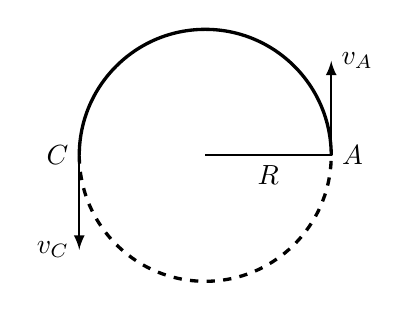
\begin{tikzpicture}[>=latex, scale=.8]
    \draw[very thick](2,0)node[right]{$A$}arc (0:180:2);
\draw[dashed,very thick](-2,0)node[left]{$C$} arc (-180:0:2);
\draw[->,thick](0,0)--node[below]{$R$}(2,0)--(2,1.5)node[right]{$v_A$};
\draw[->,thick](-2,0)--(-2,-1.5)node[left]{$v_C$};
\end{tikzpicture}
    \caption{}
    \end{minipage}
    \begin{minipage}[t]{0.48\textwidth}
    \centering
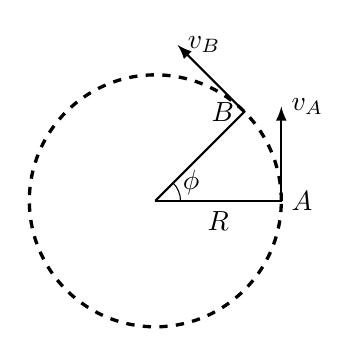
\begin{tikzpicture}[>=latex, scale=.8]
    \draw[very thick, dashed](0,0)circle(2);
    \draw[->,thick](0,0)--node[below]{$R$}(2,0)node[right]{$A$}--(2,1.5)node[right]{$v_A$};
    \draw[->,thick](0,0)--(45:2)node[left]{$B$}--+(135:1.5)node[right]{$v_B$};
    \draw(.4,0) arc (0:45:.4)node[right]{$\phi$};
\end{tikzpicture}
    \caption{}
    \end{minipage}
    \end{figure}

\end{solution}
\item 举出两个实例,说明物体做曲线运动的条件.

\begin{solution}
    如图4.12所示,一个在水平面上运动着的小球,如果
    受到一个弧形挡板的阻挡,由于挡板对小球作用的弹力$F$
的方向和小球的速度不在同一条直线上,所以小球将沿着弧
形板做曲线运动。在水平桌面上做直线运动的钢珠,如果在
它的运动路线旁边放上一根条形磁铁,钢珠就会在跟它的运
动方向不在同一直线上的磁力作用下,做曲线运动。可见物
体做曲线运动的条件是:物体具有初速度,同时受到一个跟速
度方向成角度的合外力的作用。

\begin{figure}[htp]
    \centering
    \includegraphics[scale=.5]{fig/4-12.png}
    \caption{}
\end{figure}
\end{solution}
\item 某人骑着自行车以恒定的速率驶过一段弯路,自行
车进行的是匀速运动还是变速运动?为什么?

\begin{solution}
    是变速运动。因为速度是矢量,匀速运动是指物体
    速度的大小和方向都不变的运动。而这一辆自行车虽然以恒
    定的速率行驶,但在弯路上速度的方向不断改变,所以自行车
    在弯路上行驶时不是匀速运动,而是变速运动。
\end{solution}
\end{enumerate}



\subsection{练习二}
\begin{enumerate}
	\item 降落伞在下落一定时间以后的运动是匀速的,没风的时候某跳伞员着地的速度是5.6$\ms$,现庄有风,风使他以4.0$\ms$的速度沿水平方向向东移动,他将以多大的速度着地?这个速度的方向怎样?

    \begin{solution}
        设无风时跳伞员的着地速度为$v_1$, 风的作用使他获得向东移动的速度为$v_2$, 则跳伞员的着地速度$v$是$v_1$和$v_2$这两
        个速度的合速度,如图4.13所示。
\[v=\sqrt{v^2_1+v^2_2}=\sqrt{5.6^2+4.0^2}=6.9\ms\]

        设跳伞员着地时的合速度方向偏离竖直方向的角度为$\alpha$,则
\[\tan\alpha=\frac{v_2}{v_1}=\frac{4.0}{5.6}=0.7143\qquad \alpha=35^{\circ}32'\]
    \end{solution}

\begin{figure}[htp]\centering
    \begin{minipage}[t]{0.48\textwidth}
    \centering
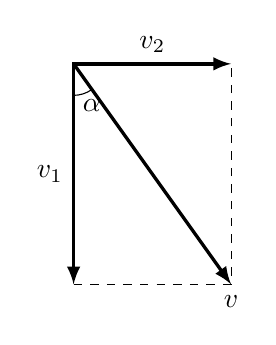
\begin{tikzpicture}[>=latex, scale=1]
\draw[<->, very thick](0,-2.8)--node[left]{$v_1$} (0,0)--node[above]{$v_2$}(2,0);
\draw[dashed](0,-2.8)--(2,-2.8)--(2,0);
\draw[->, very thick] (0,0)--(2,-2.8)node[below]{$v$};
\draw(0,-.4) arc (-90:-54.5:.4)node[below]{$\alpha$};
    \end{tikzpicture}
    \caption{}
    \end{minipage}
    \begin{minipage}[t]{0.48\textwidth}
    \centering
    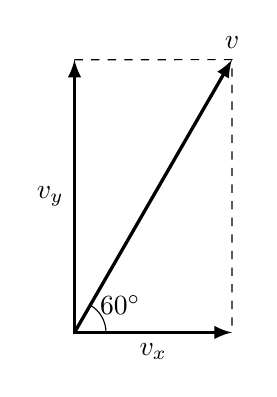
\begin{tikzpicture}[>=latex, scale=1]
\draw[<->, very thick](0,2*1.732)--node[left]{$v_y$} (0,0)--node[below]{$v_x$}(2,0);
\draw[dashed](0,2*1.732)--(60:4)--(2,0);
\draw[->, very thick] (0,0)--(60:4)node[above]{$v$};
\draw(.4,0) arc (0:60:.4)node[right]{$60^{\circ}$};
    \end{tikzpicture}
    \caption{}
    \end{minipage}
    \end{figure}

\item 炮筒与水平方向成60$^\circ$角,炮弹从炮口射出时的速度是800$\ms$.这个速度在竖直方向和水平方向的分速度各是多大?

\begin{solution}
    如图4.14所示,炮弹速度的竖直分速度
\[v_y=v\sin 60^{\circ}=800\x \frac{\sqrt{3}}{2}=693\ms\]
炮弹速度的水平分速度
\[v_x=v\cos60^{\circ}=800\x\frac{1}{2}=400\ms\]
\end{solution}
\item 小汽艇在静水中的速度是12$\kmh$,河水的流建是6.0$\kmh$.如果驾驶员向着垂直于河岸的方向驾驶,小汽艇在河水中实际行驶的速度是多大?方向怎样?

\begin{figure}[htp]
    \centering
\includegraphics[scale=.6]{fig/4-15.png}
    \caption{}
\end{figure}
\begin{solution}
    如图4.15所示,设
    小汽艇在静水中的速度$v_1=12\kmh$,由于河水的流动
    使小汽艇获得沿河流方向的速
    度$v_2=6.0\kmh$,小汽艇
    在河水中实际行驶的速度$v$是
    $v_1$和$v_2$这两个速度的合速度。
\[v=\sqrt{v_1^2+v_2^2}=\sqrt{12^2+6^2}=13.4\kmh\]
设合速度$v$和河水流动方向所成角度为$\alpha$, 则
\[\tan\alpha=\frac{v_1}{v_2}=\frac{12}{6.0}=2,\qquad \alpha=63^{\circ}26'\]
\end{solution}
\end{enumerate}

\subsection{练习三}


下面各题都不考虑空气阻力.
\begin{enumerate}
\item 从一定高度水平抛出去的物体,它在空中飞行的时间是由什么决定的?抛射的水平距离又是由什么决定的?


\begin{solution}
    由于平抛物体的运动是由水平方向的匀速直线运动
    和竖直方向的自由落体运动的合运动,则所以它在空中飞行
    的时间是由下落的距离所决定,抛射的水平距离由水平初速
    度和下落的距离决定。
\end{solution}
\item 从同一高度以不同的速度水平抛出两个质量不同的石子,下面的说法哪个对?
\begin{enumerate}
	\item 速度大的先着地;
	\item  质量大的先着地;
	\item 两个物体同时着地.
\end{enumerate}
实际做一做,看你的判断是否正确.

\begin{solution}
    由于平抛物体的飞行时间只决定于下降的高度,而
    与物体抛出的初速度和质量的大小无关。因此只有(c)说
    法是对的,即两个物体同时着地。
\end{solution}
\item 从1.6米高的地方水平射出一颗子弹,初速度是700$\ms$,求这颗子弹飞行的水平距离.

\begin{solution}
    由于下降的高度$y=\dfrac{1}{2}gt^2$. 所以飞行时间$t=\sqrt{\dfrac{2y}{g}}$。
    子弹飞行的水平距离
\[x=v_0t=v_0\sqrt{\dfrac{2y}{g}}=700\x \sqrt{\frac{2\x 1.6}{9.8}}=400{\rm m}\]
\end{solution}
\item 一个小球从1.0米高的桌面上水平抛出,落到地面的位置离开桌子的边缘2.4米,小球离开桌子边缘时的初速度多大?

\begin{solution}
小球做平抛运动的时间$t$可由公式$y=\dfrac{1}{2}gt^2$求出。
\[t=\sqrt{\frac{2y}{g}}\]
已知小球飞行的水平距离$x=2.4$米.所以
小球的平抛初速度
\[v_0=\frac{x}{t}=x\cdot \sqrt{\frac{g}{2y}}=2.4\x \sqrt{\frac{9.8}{2\x 1.0}}=5.3\ms\]
\end{solution}
\item 从15米高的楼上以1.0$\ms$的速度水平扔出一物体,此物体落地时的速度多大?方向是否与地面垂直?

\begin{solution}
    物体做平抛运动落地时的速度$v$
    是平抛初速$v_0$和在竖直方向由于重力
    作用下落15米高度时所具有的竖直分
    速度$v_y$的合速度(图4.16)。
\begin{figure}[htp]
    \centering
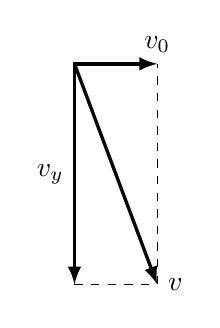
\begin{tikzpicture}[>=latex, scale=.7]
\draw[<->, very thick](1.5,0)node[above]{$v_0$}--(0,0)--node[left]{$v_y$}(0,-4);
\draw[->, very thick](0,0)--(1.5,-4)node[right]{$v$};
\draw[dashed] (0,-4)--(1.5,-4)--(1.5,0);
\end{tikzpicture}
    \caption{}
\end{figure}    
    
    由于$v^2_y=2gy$,所以物体落地时
    的合速度
\[v=\sqrt{v_0^2+v_y^2}=\sqrt{v^2_0+2gy}=\sqrt{1.0^2+2\x 9.8\x 15}=17.2\ms\]    

    方向不跟地面垂直,因为它具有水平分量。
\end{solution}
\end{enumerate}



\subsection{练习四}
    下面各题都不考虑空气阻力.
\begin{enumerate}
 \item 在斜抛运动中,射高$Y$和飞行时间$T$是由哪个分运
动决定的?

\begin{solution}
斜抛运动可以看成是水平方向的匀速直线运动和竖
直方向的上抛运动的合运动。它的飞行时间$T=2v_y/g$
,射高$Y=\dfrac{v^2_y}{2g}$。
所以射高和飞行时间都是由斜抛运动的竖直上抛分
运动所决定。
\end{solution}
 \item 在地面上以100$\ms$的初速度与水平面成60$^\circ$角
向斜上方扔出一石子.求石子在水平和竖直两个方向上的分
速度、石子能够到达的高度、到达这一高度所用的时间和石子
落地处到抛出处的距离.

\begin{solution}
    石子做斜抛运动。
    水平分速度
\[v_x=v_0\cos\theta=100\x\frac{1}{2}=50\ms\]
    竖直分速度
    \[v_y=v_0\sin\theta=100\x0.866=87\ms\]
    石子能到达的高度
    \[Y=\frac{v^2_0\sin^2\theta}{2g}=\frac{100^2\x \left(\frac{\sqrt{3}}{2}\right)^2}{2\x 9.8}=383{\rm m}\]
    石子到达最大高度所用时间
\[t=\frac{v_y}{g}=\frac{v_0\sin\theta}{g}=\frac{100\x \frac{\sqrt{3}}{2}}{9.8}=8.84{\rm s}\]
石子的飞行距离
\[X=v_0\cos\theta\cdot 2t=100\x\frac{1}{2}\x2\x8.84=884{\rm m}\]
\end{solution}
  \item 炮弹从炮筒中射出时的速度是1000$\ms$.比较炮
筒的仰角是30$^\circ$,45$^\circ$,60$^\circ$时,炮弹的射高和射程有何不同.

\begin{solution}
    炮弹作斜抛运动。

    当仰角是$\theta_1=30^{\circ}$时,
\[\begin{split}
     \text{射高}\; Y_1&=\frac{v^2_0\sin^2\theta_1}{2g}=\frac{(1000)^2\x \left(\frac{1}{2}\right)^2}{2\x 9.8}=1.28\x 10^4{\rm m}\\
     \text{射程}\; X_1&=\frac{v^2_0\sin 2\theta_1}{g}=\frac{(1000)^2\x \frac{\sqrt{3}}{2}}{ 9.8}=8.84\x 10^4{\rm m}
\end{split}
   \]
    
    当仰角是$\theta_2=45^{\circ}$时,
\[\begin{split}
     \text{射高}\; Y_2&=\frac{v^2_0\sin^2\theta_2}{2g}=\frac{(1000)^2\x \left(\frac{\sqrt{2}}{2}\right)^2}{2\x 9.8}=2.55\x 10^4{\rm m}\\
     \text{射程}\; X_2&=\frac{v^2_0\sin 2\theta_2}{g}=\frac{(1000)^2\x 1}{ 9.8}=1.02\x 10^5{\rm m}
\end{split}
   \]
    
   当仰角是$\theta_3=60^{\circ}$时,
   \[\begin{split}
        \text{射高}\; Y_3&=\frac{v^2_0\sin^2\theta_3}{2g}=\frac{(1000)^2\x \left(\frac{\sqrt{3}}{2}\right)^2}{2\x 9.8}=3.83\x 10^4{\rm m}\\
        \text{射程}\; X_3&=\frac{v^2_0\sin 2\theta_3}{g}=\frac{(1000)^2\x \frac{\sqrt{3}}{2}}{ 9.8}=8.84\x 10^4{\rm m}
   \end{split}
      \]

      由以上计算可知,射高随仰角的增大而增大,射程在仰角
为$45^{\circ}$时有最大值,而当仰角为$30^{\circ}$和$60^{\circ}$时,射程是相等的。
\end{solution}
  \item 一个人向着与水平面成45$^\circ$角的前上方抛出一颗手
榴弹.测出手榴弹的射程是65米,手榴弹抛出时的速度是多
大?射高是多高?

\begin{solution}
    手榴弹的运动是斜抛运动,忽略人的身长,则
\[X=\frac{v^2_0\sin2\theta}{g}\]
\[\begin{split}
    \text{初速}\;v_0&=\sqrt{\frac{Xg}{\sin2\theta}}=\sqrt{\frac{65\x 9.8}{\sin 90^{\circ}}}=25.2\ms\\
    \text{射高}\; Y&=\frac{v^2_0\sin^2\theta}{2g}=\frac{65\x 9.8\x \frac{1}{2}}{2\x 9.8}=16.3\ms
\end{split}\]
\end{solution}
\end{enumerate}


\subsection{练习五}
\begin{enumerate}
\item 对于做匀速圆周运动的物体,下面的哪种说法对,哪
种说法不对?
\begin{enumerate}
\item 速度不变;
\item 速率不变;
\item 角速度不变.
\end{enumerate}

\begin{solution}
    (a)不对。因为速度是矢量。线速度的方向时刻在改
    变,始终沿着圆周的切线方向。
    (b)、(c)对的。
\end{solution}
\item 钟表上分针的周期和角速度是多大?

\begin{solution}
    分针转一周的时间$T=1{\rm h}=3600{\rm s}$。
\[\text{角速度}\; \omega=\frac{2\pi}{T}=\frac{2\x 3.14}{3600}=1.74\x 10^{-3}{\rm rad/s}\]
\end{solution}
\item 半径10厘米的砂轮,每0.2秒转一圈,砂轮旋转的
角速度是多大?砂轮上离转抽不同距离的点,其角速度是否相
等?线速度是否相等?试求离转轴最远处的线速度.

\begin{solution}
    由题意可知,砂轮转动周期$T=0.2$秒,则砂轮旋转的
    角速度
    \[\omega=\frac{2\pi}{T}=\frac{2\x 3.14}{0.2}=31.4{\rm rad/s}\]
    砂轮上离轴不同距离的点的角速度是相等的,线速度则不相
    等,离转轴最远处,即砂轮边缘的点的线速度为最大,
\[v=\frac{2\pi r}{T}=\frac{2\x 3.14\x 0.10}{0.2}=3.14\ms \]
\end{solution}
\item 在皮带传动(图4.17)中,两皮带轮轮缘上的线速度
是相等的.如果大轮的半径是$r_1$,小轮的半径是$r_2$,求大
轮和小轮的角速度之比.如
果大轮每分钟的转数为$n_1$,
小轮每分钟的转数$n_2$是多少?


\begin{figure}[htp]
    \centering
    
    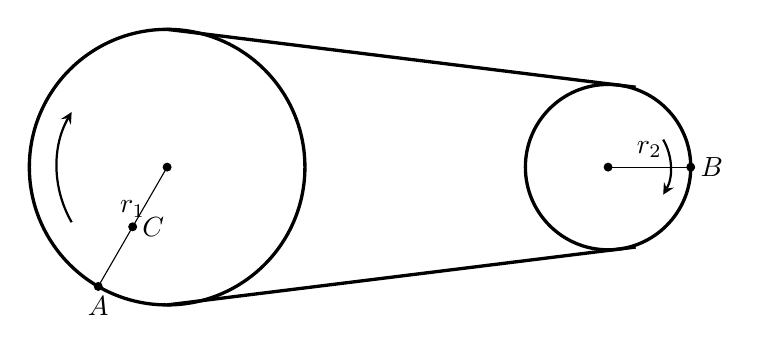
\begin{tikzpicture}[>=stealth, scale=.7]
    \draw [very thick](0,0)  circle [radius=2.5];
    \draw [very thick](8,0)  circle [radius=1.5];
    
    \draw [->, thick](210:2) arc (210:150:2);
    \draw [->, thick](9,.5) arc (30:-30:1);
    \draw (0,0)--node [above]{$r_1$}(240:2.5);
    \draw (8,0)--node [above]{$r_2$}(9.5,0);
    
    \draw [fill=black] (240:2.5) circle (2pt)node [below]{$A$};
    \draw [fill=black] (240:1.25) circle (2pt) node [right]{$C$};
    \draw [fill=black] (0,0) circle (2pt) ;
    \draw [fill=black] (8,0) circle (2pt) ;
    \draw [fill=black] (9.5,0) circle (2pt) node [right]{$B$} ;
    
    \draw [very thick] (0,2.5)--(8.5,1.45);
    \draw [very thick] (0,-2.5)--(8.5,-1.45);
    
    \end{tikzpicture}
    \caption{}
    \end{figure}

\begin{solution}    
    由于大、小两轮轮缘上的点的线速度相等,$v_1=v_2$,
    即:
    \[\omega_1 r_1=\omega_2 r_2\]
    大轮和小轮的角速度之比:
\[\frac{\omega_1}{\omega_2}=\frac{r_2}{r_1}\]

$\because\quad \omega=2\pi n$

$\therefore\quad \dfrac{n_1}{n_2}=\dfrac{\omega_1}{\omega_2}=\dfrac{r_2}{r_1}$

小轮每分钟转数$n_2=\dfrac{r_1}{r_2}n_1$.
\end{solution}
\end{enumerate}


\subsection{练习六}
\begin{enumerate}
	\item 在图4.17所示的皮带传动装置中,两轮边缘上的$A$点和$B$点的向心加速度哪个大?为什么?大轮上$A$点和$C$点的向心加速度哪个大?为什么?

    \begin{solution}
由于两轮边缘上的$A$点和$B$的线速度$v$相等,可根据$a_n=v^2/r$
式来进行比较。因为大轮半径$r_A$大于小轮半径
$r_B$, 所以向心加速度$a_B>a_A$·

由于$A$点和$C$点都是同一轮子上的点,它们的角速度$\omega$
相等,根据$a_n=\omega^2r$一式可以判断,因为半径$r_A>r_C$, 所以向
心加速度$a_A>a_C$.    
    \end{solution}
	\item 从$a_n=v^2/r$看,$a_n$跟$r$成反比,从$a_n=\omega^2r$看,$a_n$跟$r$成正比.如果有人问你:“向心加速度的大小跟半径是成正比还是成反比?”应该怎样回答?

    \begin{solution}
    任何物理量间的定量关系总是有条件的。在线速度
$v$相同的条件下,$a_n$跟$r$成反比;而在角速度$\omega$相同的条件
下,$a_n$跟$r$成正比。
    \end{solution}
	\item 由于地球的自转,地球上的物体都有向心加速度,试回答:
\begin{enumerate}
	\item “在地球表面各处的向心加速度的方向都是指向地心的”,这种说法正确吗?为什么?
	\item 在赤道和极地附近的向心加速度哪个大?为什么?
	\item 在北京的物体由于地球自转而产生的向心加速度是多大(北京的纬度取40$^\circ$,地球的半径取$6.4\times 10^8$千米)?	
\end{enumerate}

\begin{figure}[htp]
    \centering
    \includegraphics[scale=.6]{fig/4-18.png}
    \caption{}
    \end{figure}

\begin{solution}
\begin{enumerate}
    \item 不正确.如图4.18所示,在地球表面纬度为$\phi$的$P$
    处的物体,它的向心加速度的方
    向是指向做圆周运动的圆心$O$,
    而不是指向地心的。
    \item 由于在赤道上的物体和极地附近的物体随地球自转
    做圆周运动的角速度都相等,而做圆周运动的半径则是赤道大于极地附近,根据$a_n=\omega^2 r$, 所以在赤道上的物体的向心加
    速度大。
    \item 由图4.18可知,$\phi=40^{\circ}$, 圆周半径$r=R\cos\phi$, 所以
\[a_n=\omega^2r=\left(\frac{2\pi}{T}\right)^2R\cos\phi=\left(\frac{6.28}{86400}\right)^2\x6.4\x10^3\x10^3\x
    \cos40^{\circ}=2.6\x10^{-2}\msq\]
\end{enumerate}
\end{solution}
\item	 飞机由俯冲转为拉起的一段轨迹可以看作一段圆弧(图4.19).如果这段圆弧的半径$r$是800米,飞机在圆弧最低点$P$的速率为720$\kmh$.求飞机在$P$点的向心加速度是重力加速度的几倍.($g$取10$\msq$)
\begin{figure}[htp]
\centering
\includegraphics[scale=.6]{fig/4-19.png}
\caption{}
\end{figure}


\begin{solution}
    飞机在圆弧最低点$P$的速率$v=720\kmh=200\ms$.则向心加速度
   \[a_n=\frac{v^2}{r}=\frac{200^2}{800}=50\msq\]
   这时向心加速度是重力加速度的$\dfrac{50}{10}=5$倍.
\end{solution}
	\item 一个物体做匀速圆周运动,如果圆周的半径是$r$,运动的周期是$T$,试证明向心加速度$a=4\pi^2r/T$.

    \begin{solution}
        向心加速度$a=\omega^2 r$, 而角速度$\omega=2\pi/T$,
        由二式中消
        去$\omega$, 即得
        \[a=\frac{4\pi^2r}{T^2}\]
    \end{solution}
\end{enumerate}



\subsection{练习七}
\begin{enumerate}
	\item 下面的受力分析对吗?如果不对,说明错在哪里.
	\begin{enumerate}
		\item 课本图4.21中做匀速围周运动的物体受四个力的作用,这四个力是重力、支持力、绳的拉力和向心力;
		\item 课本图4.22中水平盘旋的飞机受到三个力的作用,这三个力是向心力、重力、升力.
	\end{enumerate}

    \begin{solution}
 \begin{enumerate}
     \item 不对.课本图4.21中做匀速圆周运动的物体受
     三个力的作用,这三个力是重力、支持力和绳的拉力。其中重
     力和支持力大小相等,方向相反,互相抵消,使物体做匀速圆周运动所需的向心力是绳子的拉力。
     \item 不对.课本图4.22中水平盘旋的飞机只受到重力和
     升力这两个力的作用,这两个力不在同一直线上,它们在水平
     方向的合力是使飞机水平盘旋做圆周运动所需的向心力。
 \end{enumerate}
     上面两则受力分析的共同错误是在物体所受的合外力之
     外又凭空增加了一个“向心力”。
    \end{solution}
\item 要使一个3.5千克的物体在半径是2.0米的圆周上以4.0$\ms$的速率运动,需要多大的向心力?

\begin{solution}
    物体需要的向心力
\[F=m\frac{v^2}{r}=3.5\x \frac{4.0^2}{2.0}=28{\rm N}\]
\end{solution}
\item 太阳的质量是$1.98\times 10^{30}$千克,它离开银河系中心大约3万光年(1光年$=9.46\times 10^{12}$千米),它以250千米/秒的速率绕着银河系中心转动,计算太阳绕银河系中心转动的向心力.

\begin{solution}
    太阳绕银河系中心的运动可以看成是匀速圆周运
    动,已知圆半径$r=3\x10^4\x9.46\x10^{12}\x10^3$m,$v=250\x10^3\ms$。所以向心力
\[F=m\frac{v^2}{r}=1.98\x 10^{30}\x \frac{250^2\x 10^6}{3\x 10^4\x 9.46\x 10^{15}}=4.36\x 10^{20}{\rm N}\]
\end{solution}
\item 甲乙两球都做匀速圆周运动,甲球的质量是乙球的3倍,甲球在半径是25厘米的圆周上运动,乙球在半径是16厘米的圆周上运动,在一分钟内,甲球转了30次,乙球转了75次,试比较两球所受的向心力.

\begin{solution}
    甲球的运动周期$T_1=\dfrac{60}{30}=2{\rm s}$.乙球的运动周期
    $T_2=\dfrac{60}{75}=\dfrac{4}{5}{\rm s}$。
设乙球质量为$m_2$, 则甲球质量$m_1=3m_2$。

    根据$F=m\omega^2 r=\dfrac{m4\pi^2 r}{T^2}$,
\[\frac{F_1}{F_2}=\frac{\dfrac{3m_2\x 4\pi^2\x 0.25}{2^2}}{\dfrac{m_2\x 4\pi^2\x 0.16}{\left(\frac{4}{5}\right)^2}}=\frac{3}{4}\]
    即甲球所受向心力是乙球的$3/4$
    倍。
\end{solution}
\item 线的一端拴一重物,手握线的另一端使重物在水平面内做匀速圆周运动,当每分钟转数相同时,线长易断还是线短易断?为什么?线速度相同时又怎样?

\begin{solution}
    每分钟转数相同,角速度也相等,由$F=m\omega^2r$可知-
    线长时$r$大,所需的向心力也大,所以线长容易断。而如果线
    速度相同,由$F=mv^2/r$
    可知,线短时$r$小,所需的向心力也大,
    所以线短容易断。
\end{solution}
\end{enumerate}




\subsection{练习八}
\begin{enumerate}
	\item 在课本图4.24的圆锥摆中,如果线和垂直方向成30$^\circ$角,小球在水平面内做每分钟60转的匀速圆周运动,线的长度是0.28米,计算重力加速度的值.

    \begin{solution}
        由课本图4.24可知,使圆锥摆做匀速圆周运动的向心力$F=mg\tan\theta$, 把它代入向心力公式$F=m\omega^2r$, 由于
        $r=\ell\sin\theta$, 所以$\theta$和$\omega$存在以下关系:
\[g\tan\theta=\omega^2\ell\sin\theta\]
于是,重力加速度
\[g=\omega^2\ell\cos\theta=\frac{4\pi^2}{T^2}\ell\cos\theta=\frac{4\pi^2\x 0.28\x \frac{\sqrt{3}}{2}}{1^2}=9.56\msq\]
    \end{solution}
\item 有人说:“图4.24中的圆锥摆少画了一个作用在小球上的力,这个力与$F$大小相等、方向相反,是$F$的平衡力,必须有这个力,小球才能处于平衡状态而不落向圆心.”这种说法错在哪里?

\begin{solution}
    在圆锥摆中做匀速圆周运动的小球,必须受到向心
    力的作用。正是在这个向心力的作用下产生的向心加速度,
    使速度的方向时刻发生变化,才能使小球沿着圆周运动,并不
    会使小球落向圆心,如果小球受的力是平衡的,它就不可能
    做匀速圆周运动了,物体受到的任何一个力,都不能没有施力
    物体。在圆锥摆中,小球只受到两个力,一个是地球施给它的
    重力,另一个是悬绳施给它的拉力。这两个力的合力,就是小
    球所受的向心力$F$. 此外,找不到任何其他物体能对小球施加
    一个跟$F$大小相等、方向相反的力。
\end{solution}
\item 铁路转弯处圆弧的半径是300米,轨距是1435毫米,规定火车通过这里的速度是72$\kmh$,计算内、外铁轨的高度差.
\begin{figure}[htp]
    \centering
    \includegraphics[scale=.6]{fig/4-20.png}
    \caption{}
    \end{figure}

\begin{solution}
    如图4.20所示,火车在转弯时所需的向心力由火车的重力和轨道支持力的合力F
所提供。
\[F=mg\tan\alpha=\frac{mv^2}{r},\qquad \tan\alpha=\frac{v^2}{gr}\]

由于轨道平面和水平面间的夹角$\alpha$一般较小,可以近似地认为$\tan\alpha\approx \sin\alpha=\dfrac{h}{d}$。(式中$b$为内、外轨道的高度差,$d$为
轨距)代入上式,得
\[\frac{h}{d}=\frac{v^2}{gr}\]
内、外轨道的高度差
\[h=\frac{dv^2}{gr}=\frac{1.435\x\left(\dfrac{72\x 10^3}{3600}\right)^2}{9.8\x 300}=0.195{\rm m}\]
\end{solution}
\item 一架滑翔机用180$\kmh$的速率,沿着半径为1200米的水平圆弧飞行,计算机翼和水平线的夹角(参阅课本图4.22).

\begin{solution}
    滑翔机的速率$v=180\kmh=50\ms$.滑翔机
    在水平面上做圆周运动所需的向心力是由它的重力和机翼所
    产生的升力的合力所提供.设机翼和水平面间的夹角为$\theta$, 则
    \[mg\tan\theta=\frac{mv^2}{r}\]
    \[\tan\theta=\frac{v^2}{gr}=\frac{50^2}{9.8\x 1200}=0.2126,\qquad \theta=12^{\circ}\]
\end{solution}
\end{enumerate}





\subsection{习题}

\begin{enumerate}
	\item 汽艇在静水中的速度是10$\kmh$,渡河时向着垂直于河岸的方向匀速行驶.现在河水的流速是3$\kmh$,河宽500米,汽艇驶到对岸需要多长时间?汽艇在河水中实际行驶的距离是多大?
    \begin{figure}[htp]
        \centering
        \includegraphics[scale=.6]{fig/4-21.png}
        \caption{}
        \end{figure}

    \begin{solution}
如图4.21所示,汽艇渡河时的运动是汽艇在静水中
航行的运动和由于河水冲击使汽艇沿河水流动方向的运动的
合运动,汽艇驶到对岸需要的时间
\[t=\frac{s_1}{v_1}=\frac{0.5}{10}=0.05{\rm h}=3{\rm min}\]

在这段时间里汽艇由于河水的冲击,偏向下游的距离
\[s_2=v_2t=3\x0.05=0.15{\rm km }=150{\rm m}\]
汽艇在河水中实际行驶的距离
\[s=\sqrt{s_1^2+s_2^2}=\sqrt{500^2+150^2}=522{\rm m}\]    
    \end{solution}
\item 在490米的高空,以240$\ms$的速度水平飞行的轰炸机,追击一鱼雷艇,该艇正以25$\ms$的速度与飞机同方向行驶.试问,飞机应在鱼雷艇后面多远处投下炸弹,才能击中该艇?

\begin{solution}
    飞机上投下的炸弹可看成作平抛运动。因此炸弹飞
    行时间可根据公式$h=\frac{1}{2}gt^2$来计算。
\[t=\sqrt{\frac{2h}{g}}=\sqrt{\frac{2\x 490}{9.8}}=10{\rm s}\]

由于飞机与鱼雷艇同方向行驶,所以飞机相对于鱼雷艇
的速度是$v_1-v_2=240-25=215\ms$,设飞机
在鱼雷艇后面$x$处投弹方能击中鱼雷艇,于是
\[x=(v_1-v_2)t=215\x10=2.15\x10^3{\rm m}\]
\end{solution}
\item 两人传球,如果球从一个人手里到另一个人手里经过的时间是2秒,球到达的最高点离手有多高?(设两人的手等高)

\begin{solution}
设两人间传球的运动是斜抛运动。由题意可知球做
斜抛运动的飞行时间为2秒,则球从抛出到达最高点的时间
为1秒,从最高点到达另一个人手中的时间也是1秒.由于球
到达最高点以后的运动可看成是平抛运动,于是这一最高点
离手的高度可按公式$h=\frac{1}{2}gt^2$计算。
\[h=\frac{1}{2}gt^2=\frac{1}{2}\x 9.8\x 1^2=4.9{\rm m}\]
\end{solution}
\item 从仰角是30$^\circ$的枪筒中射出的子弹,初速度是600$\ms$.求子弹在轨迹最高点和落地点的速度各是多大.

\begin{solution}
    子弹飞行到它的轨迹最高点时,由于竖直方向的速
    度已减小到零,因此这时的速度就等于斜抛初速度的水平分
    速度
    \[v_{\text{最高点}}=v_0\cos\theta=600\x \frac{\sqrt{3}}{2}=520\ms\]
    子弹到达落地点时的速度的大小等于初速度的大小,即
    \[v=v_0=600\ms\]
\end{solution}
\item 伽利略曾说过:“仰角(即抛射角)比45$^\circ$增大或减小一个相等角度的抛体,其射程是相等的.”你能证明这个说法
的正确性吗?

\begin{solution}
斜抛运动的射程
\[X=v_x T=v_0\cos\theta \x\frac{2v_0\sin\theta}{g}=\frac{2v_0^2\sin\theta\cos\theta}{g}
\]
根据伽利略的说法,设两个斜抛运动的仰角分
别为$\alpha=45^{\circ}+\theta$和$\beta=45^{\circ}-\theta$, 于是射程
\[X_1=\frac{2v_0^2\sin\alpha\cos\alpha}{g},\qquad X_2=\frac{2v_0^2\sin\beta\cos\beta}{g}\]

要证明$X_1$等于$X_2$, 只要证明$\sin\alpha\cos\alpha$ 等于 $\sin\beta \cos\beta$. 由命
题可知$\alpha +\beta =90^{\circ}$, 于是:
\[\sin\alpha\cos\alpha=\sin (90^{\circ}-\beta )\cos (90^{\circ}-\beta ) =\cos\beta \sin\beta \]
所以$X_1=X_2$. 伽利略的说法是正确的。
\end{solution}
\item 一个人站在地面上用枪踏准树上的猴子(图4.22),当子弹从枪口射出时,猴子闻声立即从树上竖直下落(初速度为零).讨论一下,猴子能否避开子弹的射击.
\begin{figure}[htp]
\centering\includegraphics[scale=.6]{fig/4-22.png}
\caption{}
\end{figure}
提示:斜抛运动可以看作是物体沿初速度方向所做的匀速直线运动和在重力作用下的自由落体运动的合运动.

\begin{figure}[htp]
    \centering\includegraphics[scale=.6]{fig/4-23.png}
    \caption{}
    \end{figure}


\begin{solution}
如图4.23所示,猴子
位于树上的$A$点,枪口$O$对准猴子。子弹射出后,如果不考
虑重力的影响,它将沿着$OA$方
向做匀速直线运动,命中$A$点。但是在重力作用下,子弹在沿
$OA$方向作匀速直线运动的同时,还要在竖直方向上作自由落
体运动。所以它在本应到达$A$点的这段时间里,只能到达$A$
点正下方的$B$点。$AB=s$就是这段时间里自由落体下降的
距离。由于猴子是在开枪的同时下落的,在同一时间里,它下
降的距离也是$s$, 恰好到达$B$点,被子弹所击中。
\end{solution}
\item  飞机从俯冲到拉起的一段轨迹是一段圆弧(参看图4.19),如果飞机在这段弧上的速率是540$\kmh$,要使它在最低点时的向心加速度不超过$5g$,圆弧的半径至少是多少米?($g$取$10\msq$).

\begin{solution}
    根据向心加速度$a_n=v^2/r$, 飞机速率$v=540\kmh=150\ms$,则圆弧半径
    \[r=\frac{v^2}{a_n}=\frac{150^2}{5g}=\frac{150^2}{5\x 10}=450{\rm m}\]
\end{solution}
\item  一个35千克的重物,系在2.0米长的悬绳下端,不断摆动.重物通过最低点时的速率是3.0$\ms$,求这时绳对物体的拉力.

\begin{solution}
    重物的摆动可以看作是在竖直平面里的圆周运动的一部分。当重物经过圆周最低
    点时,受到的重力$mg$和绳子
    拉力$T$的合力应等于重物作
    圆周运动所需的向心力(图
    4.24)。
\[T-mg=ma\]
于是,绳子拉力
\[T=mg+ma=m\left(g+\frac{v^2}{r}\right)=35\left(9.8+\frac{3.0^2}{2.0}\right)=5.0\x 10^2{\rm N}\]
\end{solution}

\begin{figure}[htp]\centering
    \begin{minipage}[t]{0.48\textwidth}
    \centering
\begin{tikzpicture}[>=latex]
\fill [pattern=north east lines](-.5,3) rectangle (.5,3.2);
\draw(-.5,3)--(.5,3); \draw(0,3)--(0,0);
\draw(0,0) arc (-90:-60:3); \draw(0,0) arc (-90:-120:3);
\draw[fill=white](0,0) circle (.2);
\draw[<->, thick](0,1)node[right]{$T$}--(0,-1)node[right]{$mg$};
\draw[->](-.2,.3)--(-.7,.3)node[above]{$v$};
\tkzDefPoints{0/0/O} \tkzDrawPoint(O)
\end{tikzpicture}
    \caption{}
    \end{minipage}
    \begin{minipage}[t]{0.48\textwidth}
    \centering
    \includegraphics[scale=.7]{fig/4-25.png}
    \caption{}
    \end{minipage}
    \end{figure}

\item  略(课本已作解答).

\item  一个滑雪者连同他的滑雪板质量共70千克,他滑到凹形的坡底时的速度是20$\ms$,坡底的圆弧半径是50米,计算在坡底时雪地对滑雪板的支持力.

\begin{solution}
    滑雪者滑到凹形坡底时所需的向心力是由坡底对滑
    雪板的支持力N和滑雪者连同滑雪板的重力$mg$的合力所
    提供,
\[    N-mg=ma\]
    所以,坡底雪地的支持力
\[N=mg+ma=m\left(g+\frac{v^2}{r}\right)=70\left(9.8+\frac{20^2}{50}\right)=1.2\x 10^3{\rm N}\]
\end{solution}
\item  一辆600千克的汽车以10$\ms$的速度通过圆弧半径是30米的山坡顶点时,汽车受到哪几个力的作用?汽车对路面的压力是多大?


\begin{solution}
    汽车通过山坡顶点时受
    到重力$mg$和山坡顶点的支
    持力$N$的作用,这两个力的合
    力等于汽车在竖直平面里做圆
    周运动所需的向心力(图4.25)。
\[mg-N=\frac{mv^2}{r}\]
\[N=m\left(g-\frac{v^2}{r}\right)=600\left(9.8-\frac{10^2}{30}\right)=3.88\x 10^3{\rm N}\]
汽车对路面的压力也等于$3.88\x10^3$牛.
\end{solution}

\end{enumerate}


\section{参考资料}
\subsection{对课本170页习题第6题提示的讨论}
这是研究斜抛运动时常用的一种分析方法。可以这样来
设想,如果不存在重力和其他任何力的作用,根据牛顿第一定
律可知,物体将以斜抛时的初速度沿着抛出方向做匀速直线
运动,又根据力的独立作用原理可知,对物体作用的任何一
个力都要使物体产生加速度,若不计空气阻力的影响,则斜抛
物体只受到重力的作用,重力使物体产生的加速度等于$g$, 从
而使物体在竖直方向上发生速度的改变,在时间$\Delta t$内,物体
的速度变化$\Delta v=g\Delta t$.

投某一斜抛物体的初速度$v_0=40\ms$,抛射角$\theta=30^{\circ}$,
$g$取$10\msq$, 则初速度的竖直分速度
$$v_y=v_0\sin\theta=40\x\frac{1}{2}=20\ms$$
物体上升到最大高度的时间
\[t=\frac{v_0\sin\theta}{g}=\frac{20}{10}=2{\rm s}\]
飞行时间$T=2t=2\x2=4{\rm s}$,即物体抛出后运动4秒就
落到地面。可以这样来想象,如果没有重力的作用,在4秒末
物体将运动到哪里呢?从图4.26可以看出,物体如果以初速
$v_0$做匀速直线运动,则4秒内的位移$OD=v_0t=40\x4=
160{\rm m}$。从图中直角三角形$ODH$来看,对边$DH=OD\sin\theta=
160\x\frac{1}{2}=80{\rm m}$,即物体应在离地面80米高处的$D$点,然
而事实上物体却在重力作用下落到了地面,因为根据自由落
体运动可知
\[y=\frac{1}{2}gt^2=\frac{1}{2}\x 10\x 4^2=80{\rm m}\]
这表明了在
这4秒时间内,由于重力作用使物体下降的距离恰为80米,
所以物体恰好落回到地面。

\begin{figure}[htp]\centering
    \begin{minipage}[t]{0.58\textwidth}
    \centering
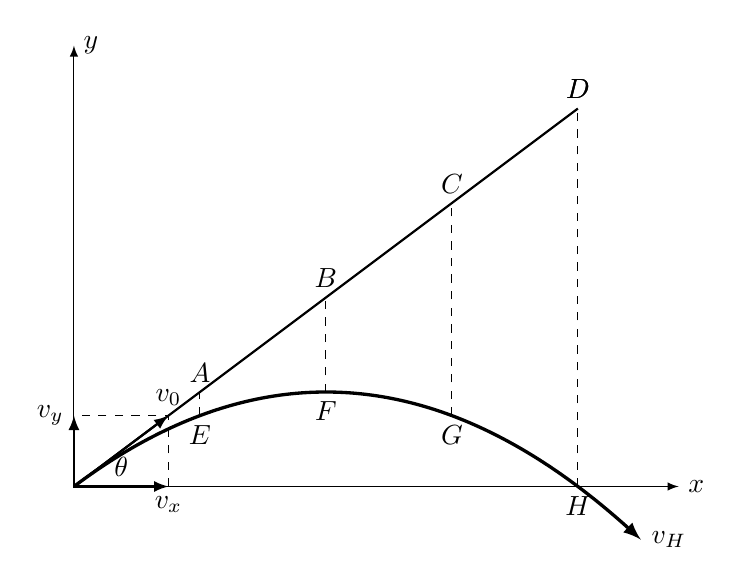
\begin{tikzpicture}[>=latex, scale=.8]
    \draw[<->](0,7)node[right]{$y$}--(0,0)--(9.6,0)node[right]{$x$};
\draw[thick](0,0)--(8,6)node[above]{$D$};
\draw[domain=0:9, samples=100,very thick,->]plot(\x, {-5/53.33*\x*\x+.75*\x})node[right]{$v_H$};
\draw[dashed](2,1.125)node[below]{$E$}--(2,1.5)node[above]{$A$};
\draw[dashed](4,1.5)node[below]{$F$}--(4,3)node[above]{$B$};
\draw[dashed](6,1.125)node[below]{$G$}--(6,4.5)node[above]{$C$};
\draw[dashed](8,0)node[below]{$H$}--(8,6)node[above]{$D$};

\draw[thick,<->] (1.5,0)node[below]{$v_x$}--node[above]{$\theta$}  (0,0)--(0,1.5*.75)node[left]{$v_y$};
\draw[dashed](1.5,0)-- (1.5,1.5*.75)--(0,1.5*.75);
\draw[thick,->]  (0,0)--(1.5,1.5*.75)node[above]{$v_0$};
\end{tikzpicture}
    \caption{}
    \end{minipage}
    \begin{minipage}[t]{0.38\textwidth}
    \centering
\begin{tikzpicture}[>=latex, thick]
\tkzDefPoints{-1/0/O, 2/2/A, 2/1/E, 2/0/F, 2/-1/G, 2/-2/H}
\draw[->](O)--node[above]{$v_0$}(A);
\draw[->](O)--node[above]{$v_E$}(E);
\draw[->](O)--node[above]{$v_F$}(F);
\draw[->](O)--node[below]{$v_G$}(G);
\draw[->](O)--node[below]{$v_H$}(H);
\draw[->](A)--node[right]{$\Delta v$}(E);
\draw[->](E)--node[right]{$\Delta v$}(F);
\draw[->](F)--node[right]{$\Delta v$}(G);
\draw[->](G)--node[right]{$\Delta v$}(H);
\end{tikzpicture}
    \caption{}
    \end{minipage}
    \end{figure}

根据同样的道理,可以证明距离$AE$, $BF$和$CG$分别是在
1秒内,2秒内和3秒内由于重力的作用在竖直方向上下降的
距离,显然,$AE:BF:CG:DH=1:4:9:16$, 这就说明了斜抛运
动的确可以看成是物体沿初速度方向所做的匀速直线运动和
在重力作用下的自由落体运动的合运动。

此外,可以算出每1秒内的速度改变量,$\Delta v=g\Delta t=10\x
1=10\ms$,而且$\Delta v$的方向都是竖直向下的。可以把从开始抛出
时的初速度$v_0$经过4秒钟变化到落
地点的速度$v_H$的过程用图4.27表示
出来。

\subsection{关于竖直平面内的圆周运动}

在竖直平面内做圆周运动的物体,当一经过其轨迹
的最低点时,如课本171页第8题所要讨论的情况,圆心的
位置恰在物体的正上方,所以
物体所需的向心力(也就是物
体所受到的合外力)的方向,应
是竖直向上的。但由于重力方
向总是竖直向下的,在这一位
置,重力不可能起向心力的作
用,因此向心力必须由迫使物
体做圆周运动的另一物体——
悬绳来提供.如图4.28所示,如
果物体的质量为$m$, 悬绳长$\ell$, 经过最低点时的速率为$v$, 则在这一瞬时,
\[T-mg=ma_n=\frac{mv^2}{\ell}\]
绳子拉力
\[T=m\left(g+\frac{v^2}{\ell}\right)\]
表明了在这一瞬时,绳子的拉
力除了克服物体的重力外,还要承担由于提供物体做圆周运
动所需的向心力,因此绳子的拉力必然比物体静止时要大,而
且速率$v$越大,绳子拉力也越大。

\begin{figure}[htp]\centering
    \begin{minipage}[t]{0.48\textwidth}
    \centering
\begin{tikzpicture}[>=latex]
\fill [pattern=north east lines](-.5,3) rectangle (.5,3.2);
\draw(-.5,3)--(.5,3); \draw(0,3)--(0,0);
\draw(0,0) arc (-90:-60:3); \draw(0,0) arc (-90:-120:3);
\draw[fill=white](0,0) circle (.2);
\draw[<->, thick](0,1)node[right]{$T$}--(0,-1)node[right]{$mg$};
\draw[->](-.2,-.3)--node[below]{$v$}(-.7,-.3);
\tkzDefPoints{0/0/O} \tkzDrawPoint(O)
\draw[dashed](0,3)--node[right]{$\ell$}+(-70:3)[fill=white] circle (.2);
\end{tikzpicture}
    \caption{}
    \end{minipage}
    \begin{minipage}[t]{0.48\textwidth}
    \centering
    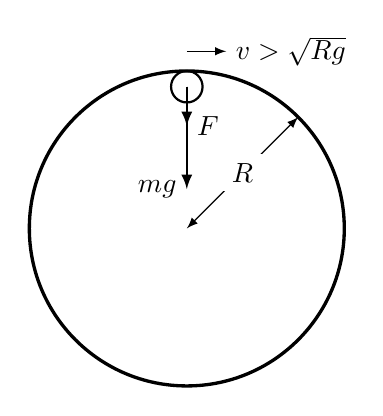
\begin{tikzpicture}[>=latex, scale=1]
\draw[very thick](0,0) circle (2);
\draw[<->](0,0)--node[fill=white]{$R$}(45:2);     
\draw[thick](0,1.8) circle (.2);
\draw[->,thick] (0,1.8)--(0,1.3)node[right]{$F$};
\draw[->,thick] (0,1.8)--(0,.5)node[left]{$mg$};
\draw[->] (0,2.25)--(.5,2.25)node[right]{$v>\sqrt{Rg}$};

    \end{tikzpicture}
    \caption{}
    \end{minipage}
    \end{figure}
在铁路和公路的立体叉道口,汽车往往是由隧道通过道
口,当汽车驶过隧道时,可以看成是在竖直平面里做圆周运
动。根据以上的分析,这时隧道底部路面受到的压力将大于汽
车重量。

当物体经过竖直圆周的最高点时,如课本图
4.33所讨论的情况,表明存在着一个最小速率$v=\sqrt{Rg}$, 式
中$R$为圆半径。如果物体的速率$v>\sqrt{Rg}$, 则所需的向心力
将大于物体所受的重力,这时,
除了物体的重力全部用作向心
力外,其不足的部分需要由圆
环顶部提供,如图4.29所示,即,
\[\frac{mv^2}{R}=mg+F\]
于是圆环顶部所受的压力
\[F'=-F=-\left(\frac{mv^2}{R}-mg\right)=-\frac{mv^2}{R}+mg\]

式中负号表示圆环顶部所受压力的方向和$F$的方向
相反。

\begin{figure}[htp]
    \centering
    \includegraphics[scale=.7]{fig/4-30.png}
    \caption{}
\end{figure}

汽车驶过一般拱形桥的顶部时,也可以看成是在竖直平
面里做圆周运动,如图4.30所示。在这一瞬时,圆心位置恰
在汽车的正下方。汽车做圆周运动经过这一位置时所需的向
心力的方向是竖直向下的,因此这一向心力就可以由汽车重
力的一部分来提供,正因为重力被用去一部分产生向心加速
度,因此作用于拱桥顶部的压力就减小了。即
\[mg-N=\frac{mv^2}{R}\]
桥顶所受的压力
\[F'=-N=-\left(mg-\frac{mv^2}{R}\right)=-mg+\frac{mv^2}{R}\]
式中负号表示拱桥顶所受的压力的方向和支持力$N$的方向
相反。

在汽车的速率$0<v<\sqrt{Rg}$的范围内,桥顶所受的压力
将比汽车静止在桥顶时要小,随着汽车行驶速率的增大,桥顶
所受的压力将减得更小,而当速率$v=\sqrt{Rg}$时,汽车做圆周
运动所需的向心力增大到恰好等于汽车所受的重力,于是桥
顶所受的压力将等于零。

如果速率$v>\sqrt{Rg}$, 则因为没有足够的向心力,汽车就
将飞离桥顶不再沿着拱桥做圆周运动。

可见以上讨论的虽然都是物体在竖直平面内做圆周运动
经过最高点时的情况,但还是有区别的,课本171页第9题
所讨论的是小球在圆弧的内侧运动,因此小球的速率必须满
足$v\ge \sqrt{Rg}$的条件,才能使小球在竖直平面里做圆周运动,
圆环顶部只有在$v>\sqrt{Rg}$的情况下才会受到压力的作用,而
在汽车驶过拱形桥顶的例子中,由于汽车在圆弧的外侧运动,
汽车的速率必须满足$v\le \sqrt{Rg}$的条件,才能使汽车沿着拱形
桥面顶部的圆弧运动,在$0<v<\sqrt{Rg}$的速率范围内,桥顶
都将受到压力的作用。

竖直平面里的圆周运动一般不是匀速圆周运动。
物体在竖直平面里做圆周运动时,由于物体所受重力的
大小和方向都是恒定不变的,因此,当物体经过圆周上的各
个不同位置时,重力对物体做圆周运动所需的向心力是否能
做出贡献、以及贡献的程度如何都是不相同的.从课本160
页的阅读材料的分析可知,假定图4.23甲所示的曲线是竖直
平面里的一段圆弧,又假定图示中的力$F$就是物体所受的重
力,这样就可想象在这一位置上,只有重力的一个垂直于圆弧
切线方向的分力$F_n$, 才起了向心力——即产生向心加速度的
作用,而重力的另一个沿着圆弧切线方向的分力$F_t$, 则起了
产生切向加速度的作用,这样,物体的线速度大小将会发生改
变,所以说一般说来,在竖直平面里的圆周运动不是匀速圆周
运动。

